\chapter{External specification}
\begin{itemize}
\item hardware and software requirements
\item installation procedure
\item activation procedure
\item types of users
\item user manual
\item system administration
\item security issues
\item example of usage
\item working scenarios (with screenshots or output files)
\end{itemize}



 
\begin{figure}
\centering
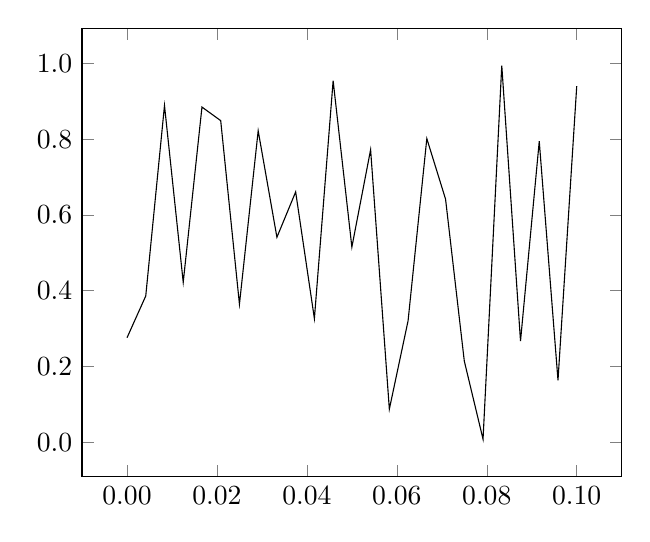
\begin{tikzpicture}
\begin{axis}[
    y tick label style={
        /pgf/number format/.cd,
            fixed,    
            fixed zerofill, % 1.0 zamiast 1
            precision=1,
        /tikz/.cd
    },
    x tick label style={
        /pgf/number format/.cd,
            fixed,
            fixed zerofill,
            precision=2,
        /tikz/.cd
    }
]
\addplot [domain=0.0:0.1] {rnd};
\end{axis} 
\end{tikzpicture}
\caption{Figure caption (below the figure).}
\label{fig:2}
\end{figure}

%%%%%%%%%%%%%%%%%%%%%
% FIGURE FROM FILE
%
%\begin{figure}
%\centering
%
\includegraphics[width=0.5\textwidth]{./graf/politechnika_sl_logo_bw_pion_en.pdf}
%\caption{Caption of a figure is always below the figure.}
%\label{fig:label}
%\end{figure}
%Fig. \ref{fig:label} presents …
%%%%%%%%%%%%%%%%%%%%%
%
%%%%%%%%%%%%%%%%%%%%
%% SUBFIGURES
%
%\begin{figure}
%\centering
%\begin{subfigure}{0.4\textwidth}
%    
\includegraphics[width=\textwidth]{./graf/politechnika_sl_logo_bw_pion_en.pdf}
%    \caption{Upper left figure.}
%    \label{fig:upper-left}
%\end{subfigure}
%\hfill
%\begin{subfigure}{0.4\textwidth}
%    
\includegraphics[width=\textwidth]{./graf/politechnika_sl_logo_bw_pion_en.pdf}
%    \caption{Upper right figure.}
%    \label{fig:upper-right}
%\end{subfigure}
%
%\begin{subfigure}{0.4\textwidth}
%    
\includegraphics[width=\textwidth]{./graf/politechnika_sl_logo_bw_pion_en.pdf}
%    \caption{Lower left figure.}
%    \label{fig:lower-left}
%\end{subfigure}
%\hfill
%\begin{subfigure}{0.4\textwidth}
%    
\includegraphics[width=\textwidth]{./graf/politechnika_sl_logo_bw_pion_en.pdf}
%    \caption{Lower right figure.}
%    \label{fig:lower-right}
%\end{subfigure}
%        
%\caption{Common caption for all subfigures.}
%\label{fig:subfigures}
%\end{figure}
%Fig. \ref{fig:subfigures} presents very important information, eg. Fig. \ref{fig:upper-right} is an upper right subfigure.
%%%%%%%%%%%%%%%%%%%%%
